\large Schreibe ein Python-Script, das einen zufälligen Parcour über das Lavabecken generiert.
\begin{itemize}
	\item Um das Lavabecken und den restlichen Rahmen zu generieren, öffne das Initiliasierungsscript \texttt{lava\_runner\_initialiser.py} und führe es aus.
	
	\item Öffne die Datei \texttt{lava\_runner.py} mit dem Editor. Diese Datei enthält bereits Code und muss lediglich im gekennzeichneten Bereich erweitert werden.
	
	\item Die Funktion \texttt{generate\_parcour} bekommt die Koordinaten (\texttt{x, y, z}) übergeben. Die Koordinaten geben die Position des Blocks an auf dem ihr steht, wenn ihr \texttt{lava\_runner.py} ausführt. Ausgehend von dieser Position soll der zufällige Parcour über das Lavabecken gebaut werden.
	
	\item Außerhalb von \texttt{generate\_parcour} gibt es zwei Variablen \texttt{x\_boundary} und \texttt{z\_boundary}. Diese geben den Rand der Arena an.
	
	\item In \texttt{generate\_parcour}: Schreibe eine Schleife, die solange läuft, wie \texttt{x} und \texttt{z} nicht den Rand der Arena überschreiten.
	
	\item  Setze mit \texttt{setBlock(x, y, z, block.ICE)} den nächsten Block des zufälligen Parcours.
	
	\item Als nächstes muss die Position für den nächsten Block bestimmt werden. Mit Hilfe der Funktion \texttt{random.randint(unter\_grenze, obere\_grenze)} könnt ihr euch einen zufälligen Wert zwischen den angegeben Grenzen geben lassen. Überlege wie die neuen Werte \texttt{x2, y2} und \texttt{z2} aussehen könnten und wähle die Grenzen \texttt{untere\_grenze, obere\_grenze} demnentsprechend. Achte darauf, dass man den neuen Block mit einem Sprung vom vorherigen Block aus erreichen können muss. Du kannst dafür die Abbildung weiter unten zur Hilfe nehmen.
	
	\item Ist die neue Position \texttt{(x2, y2, z2)} vom vorherigen Block aus erreichbar, überschreibe \texttt{(x, y, z)} mit \texttt{(x2, y2, z2)}. Ist die neue Position allerdings nicht erreichbar, dann könnt ihr mit dem Schlüsselwort \texttt{continue} dafür sorgen, dass neue Werte für \texttt{x2, y2} und \texttt{z2} ausgewählt werden.

\end{itemize}
\begin{figure}
\centering
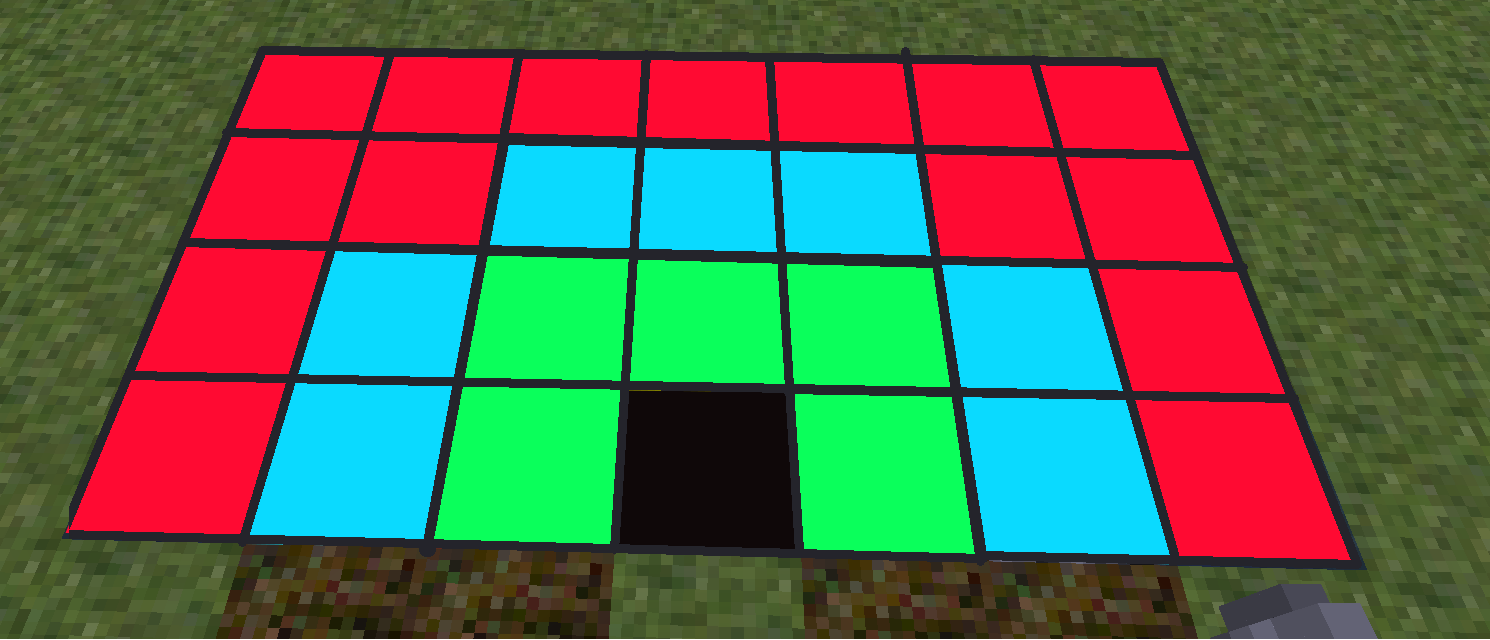
\includegraphics[scale=0.25]{src/lava_runner/res/1layer.png}
\caption{Das schwarz markierte Feld stellt die Position des vorherigen Blocks dar, die roten Felder sind nicht erreichbar, weshalb ein Block verworfen werden soll, falls er zufällig auf diesem Feld platziert werden soll.}
\end{figure}
